%%%%%%%%%%%%%%%%%%%%%%%%%%%%%%%%%%%%%%%%%
% Structured General Purpose Assignment
% LaTeX Template
%
% This template has been downloaded from:
% http://www.latextemplates.com
%
% Original author:
% Ted Pavlic (http://www.tedpavlic.com)
%
% Note:
% The \lipsum[#] commands throughout this template generate dummy text
% to fill the template out. These commands should all be removed when 
% writing assignment content.
%
%%%%%%%%%%%%%%%%%%%%%%%%%%%%%%%%%%%%%%%%%

%----------------------------------------------------------------------------------------
% PACKAGES AND OTHER DOCUMENT CONFIGURATIONS
%----------------------------------------------------------------------------------------

\documentclass{article}

\usepackage{fancyhdr} % Required for custom headers
\usepackage{lastpage} % Required to determine the last page for the footer
\usepackage{extramarks} % Required for headers and footers
\usepackage{graphicx} % Required to insert images
\usepackage{lipsum} % Used for inserting dummy 'Lorem ipsum' text into the template
\usepackage{amsmath, amsfonts, bm, physics}
\usepackage{xcolor}
\usepackage{listings}
\usepackage{hyperref}
\usepackage[toc,page]{appendix}
\usepackage{steinmetz}

\lstset{
    %numbers=left,
    stepnumber=1,    
    firstnumber=1,
    numberfirstline=true,
    basicstyle=\ttfamily,
    keywordstyle=\color{blue}\ttfamily,
    stringstyle=\color{red}\ttfamily,
    commentstyle=\color{green}\ttfamily,
    breaklines=true,
}

% Margins
\topmargin=-0.45in
\evensidemargin=0in
\oddsidemargin=0in
\textwidth=6.5in
\textheight=9.0in
\headsep=0.25in 

\linespread{1.1} % Line spacing

% Set up the header and footer
\pagestyle{fancy}
\lhead{\hmwkAuthorName} % Top left header
\chead{\hmwkClass\: \hmwkTitle} % Top center header
\rhead{\firstxmark} % Top right header
\lfoot{\lastxmark} % Bottom left footer
\cfoot{} % Bottom center footer
\rfoot{Page\ \thepage\ of\ \pageref{LastPage}} % Bottom right footer
\renewcommand\headrulewidth{0.4pt} % Size of the header rule
\renewcommand\footrulewidth{0.4pt} % Size of the footer rule

\setlength\parindent{0pt} % Removes all indentation from paragraphs

%----------------------------------------------------------------------------------------
% DOCUMENT STRUCTURE COMMANDS
% Skip this unless you know what you're doing
%----------------------------------------------------------------------------------------

% Header and footer for when a page split occurs within a problem environment
\newcommand{\enterProblemHeader}[1]{
  \nobreak\extramarks{#1}{#1 continued on next page\ldots}\nobreak
  \nobreak\extramarks{#1 (continued)}{#1 continued on next page\ldots}\nobreak
}

% Header and footer for when a page split occurs between problem environments
\newcommand{\exitProblemHeader}[1]{
  \nobreak\extramarks{#1 (continued)}{#1 continued on next page\ldots}\nobreak
  \nobreak\extramarks{#1}{}\nobreak
}

\setcounter{secnumdepth}{0} % Removes default section numbers
\newcounter{homeworkProblemCounter} % Creates a counter to keep track of the number of problems

\newcommand{\homeworkProblemName}{}
\newenvironment{homeworkProblem}[1][Problem \arabic{homeworkProblemCounter}]{ % Makes a new environment called homeworkProblem which takes 1 argument (custom name) but the default is "Problem #"
    \stepcounter{homeworkProblemCounter} % Increase counter for number of
% problems
    \renewcommand{\homeworkProblemName}{#1} % Assign \homeworkProblemName the
% name of the problem
    \section{\homeworkProblemName} % Make a section in the document with the
% custom problem count
    \enterProblemHeader{\homeworkProblemName} % Header and footer within the
% environment
}{
    \exitProblemHeader{\homeworkProblemName} % Header and footer after the
% environment
}

\newcommand{\problemAnswer}[1]{ % Defines the problem answer command with the content as the only argument
    \noindent\textbf{\emph{Answer: }}#1 % Just put a keyword Answer in
    % bold/italic at the beginning
}

\newcommand{\homeworkSectionName}{}
\newenvironment{homeworkSection}[1]{ % New environment for sections within homework problems, takes 1 argument - the name of the section
    \renewcommand{\homeworkSectionName}{#1} % Assign \homeworkSectionName to the
% name of the section from the environment argument
    \subsection{\homeworkSectionName} % Make a subsection with the custom name
% of the subsection
    \enterProblemHeader{\homeworkProblemName\ [\homeworkSectionName]} % Header
% and footer within the environment
}{
    \enterProblemHeader{\homeworkProblemName} % Header and footer after the
% environment
}

\newtheorem{theorem}{Theorem}[homeworkProblemCounter]
\newtheorem{lemma}[theorem]{Lemma}
\newtheorem{proposition}[theorem]{Proposition}
\newtheorem{corollary}[theorem]{Corollary}

\newenvironment{proof}[1][Proof]{
  \begin{trivlist}
    \item[\hskip \labelsep {\bfseries #1}]}{
  \end{trivlist}
}
\newenvironment{definition}[1][Definition]{
  \begin{trivlist}
    \item[\hskip \labelsep {\bfseries #1}]}{
  \end{trivlist}
}

\newenvironment{example}[1][Example]{
  \begin{trivlist}
    \item[\hskip \labelsep {\bfseries #1}]}{
  \end{trivlist}
}
    
\newenvironment{remark}[1][Remark]{
  \begin{trivlist}
    \item[\hskip \labelsep {\bfseries #1}]}{
  \end{trivlist}
}

\newcommand{\qed}{
  \nobreak \ifvmode \relax \else
  \ifdim\lastskip<1.5em \hskip-\lastskip
  \hskip1.5em plus0em minus0.5em \fi \nobreak
  \vrule height0.75em width0.5em depth0.25em\fi
}

\lstset{
  frame=single,
  breaklines=true,
  postbreak=\raisebox{0ex}[0ex][0ex]{\ensuremath{\color{red}\hookrightarrow\space}}
}
   
%----------------------------------------------------------------------------------------
% NAME AND CLASS SECTION
%----------------------------------------------------------------------------------------

\newcommand{\hmwkTitle}{Assignment\ \#3} % Assignment title
\newcommand{\hmwkDueDate}{Monday, May\ 16,\ 2016} % Due date
\newcommand{\hmwkClass}{MAT\ 280} % Course/class
\newcommand{\hmwkClassTime}{MF 13:30 - 15:00} % Class/lecture time
\newcommand{\hmwkClassInstructor}{Prof. Thomas Strohmer} % Teacher/lecturer
\newcommand{\hmwkAuthorName}{Wenhao Wu} % Your name

%----------------------------------------------------------------------------------------
% TITLE PAGE
%----------------------------------------------------------------------------------------

\title{
  \vspace{2in}
  \textmd{\textbf{\hmwkClass:\ \hmwkTitle}}\\
  \normalsize\vspace{0.1in}\small{Due\ on\ \hmwkDueDate}\\
  \vspace{0.1in}\large{\textit{\hmwkClassInstructor\ \hmwkClassTime}}
  \vspace{3in}
}

\author{\textbf{\hmwkAuthorName}}
\date{} % Insert date here if you want it to appear below your name

%----------------------------------------------------------------------------------------

\begin{document}

  \maketitle
  
  %----------------------------------------------------------------------------------------
  % TABLE OF CONTENTS
  %----------------------------------------------------------------------------------------
  
  %\setcounter{tocdepth}{1} % Uncomment this line if you don't want subsections listed in the ToC
  
  \newpage
  \tableofcontents
  \newpage
  
  %----------------------------------------------------------------------------------------
  % PROBLEM 1
  %----------------------------------------------------------------------------------------
  \begin{homeworkProblem}
    Download the dataset \texttt{crescents.mat} from the Class website and load
    it into Matlab. It contains two-hundred points in two dimensions. If you
    plot it, you see that the data form two half-moon-like clusters. Clearly,
    k-means directly applied to this dataset will fail to cluster the data
    according to these two shapes. Use the graph Laplacian or diffusion maps
    (followed by k-means) to try to cluster the data as good as possible
    according to the half-moon shapes. You can use Matlab’s k-means function to
    do the actual clustering once you transformed the data.
    \vspace{10pt}
      
    \problemAnswer{
      We tried to cluster the data using graph Laplacian where
      the weighted adjacency matrix $\mathbf{W}$ is evaluated with
      $\epsilon=0.001$, $0.01$ and $0.1$, respectively. When $\epsilon=0.001$
      (Fig.~\ref{fig:hw3_1_0001}), spectral clustering fails as the entries of
      the second eigenvector of $\mathbf{L}$ concentrates around 0. This is
      because $\epsilon$ is so small that almost no two points are considered to be
      close to each other. On the other hand, when $\epsilon=0.1$
      (Fig.~\ref{fig:hw3_1_01}), the spectral clustering fails again since for
      large $\epsilon$ the points that are rather far apart are still considered
      as neighbors. When $\epsilon=0.01$ (Fig.~\ref{fig:hw3_1_001}), we can see
      that the points within each ``arc'' are close to one another while the
      points from the two different ``arcs'' are far apart. As a result,
      $\mathbf{v}_2$ concentrates into two spikes and the two ``arcs'' are
      clearly separated by k-means algorithm.
      
      \begin{figure}[htb]
        \centering
        \begin{minipage}[b]{0.32\columnwidth}
          \centering
          \centerline{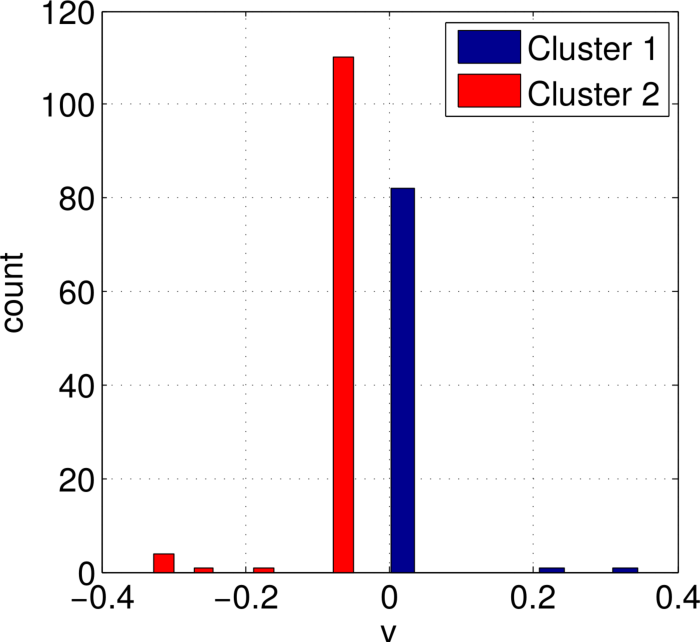
\includegraphics[width=5cm]{./figs/hw3_1_hist_0001.pdf}}
          \centerline{(a) Histogram of $\mathbf{v}_2$.}\medskip
        \end{minipage}
        \hfill
        \begin{minipage}[b]{0.32\columnwidth}
          \centering
          \centerline{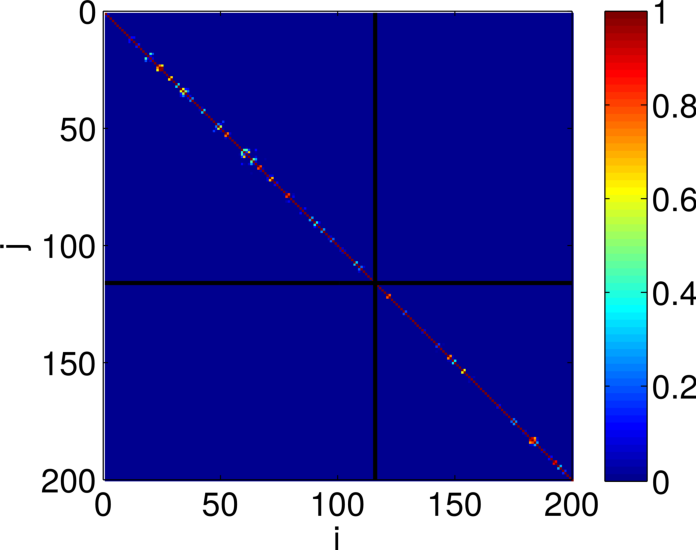
\includegraphics[width=6cm]{./figs/hw3_1_W_0001.pdf}}
          \centerline{(b) $\mathbf{W}$ ordered and clustered.}\medskip
        \end{minipage}
        \hfill
        \begin{minipage}[b]{0.32\columnwidth}
          \centering
          \centerline{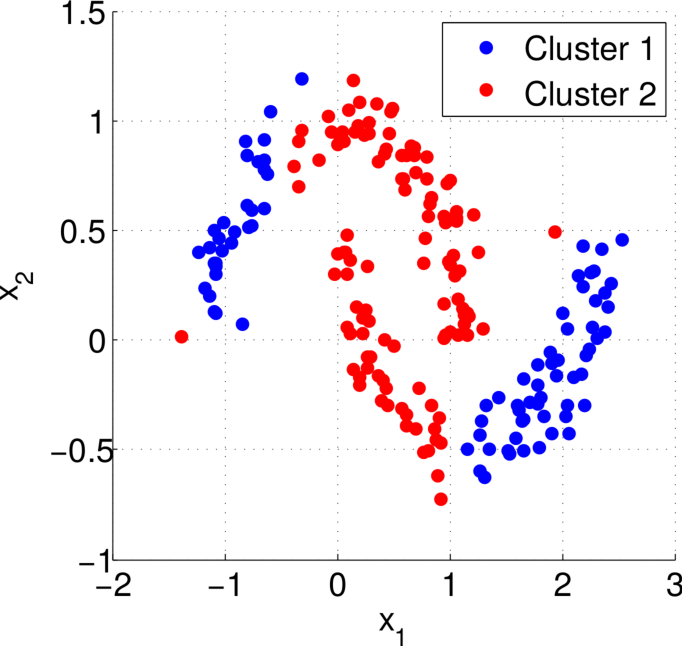
\includegraphics[width=5cm]{./figs/hw3_1_cluster_0001.pdf}}
          \centerline{(c) Clustering.}\medskip
        \end{minipage}
        \caption{Clustering result for $\epsilon=0.001$.}
        \label{fig:hw3_1_0001}
      \end{figure}
      
      \begin{figure}[htb]
        \centering
        \begin{minipage}[b]{0.32\columnwidth}
          \centering
          \centerline{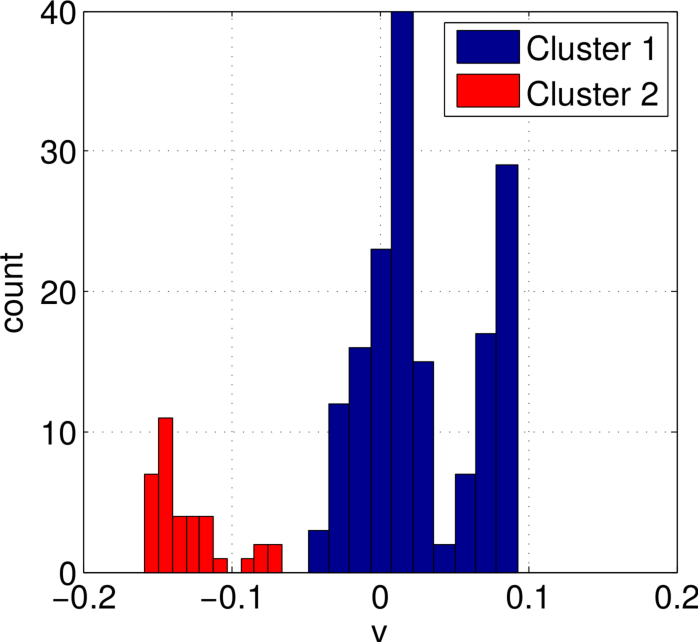
\includegraphics[width=5cm]{./figs/hw3_1_hist_01.pdf}}
          \centerline{(a) Histogram of $\mathbf{v}_2$.}\medskip
        \end{minipage}
        \hfill
        \begin{minipage}[b]{0.32\columnwidth}
          \centering
          \centerline{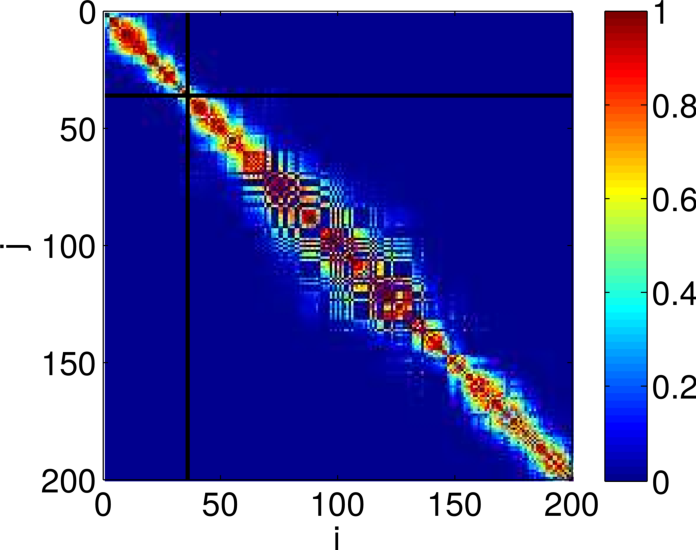
\includegraphics[width=6cm]{./figs/hw3_1_W_01.pdf}}
          \centerline{(b) $\mathbf{W}$ ordered and clustered.}\medskip
        \end{minipage}
        \hfill
        \begin{minipage}[b]{0.32\columnwidth}
          \centering
          \centerline{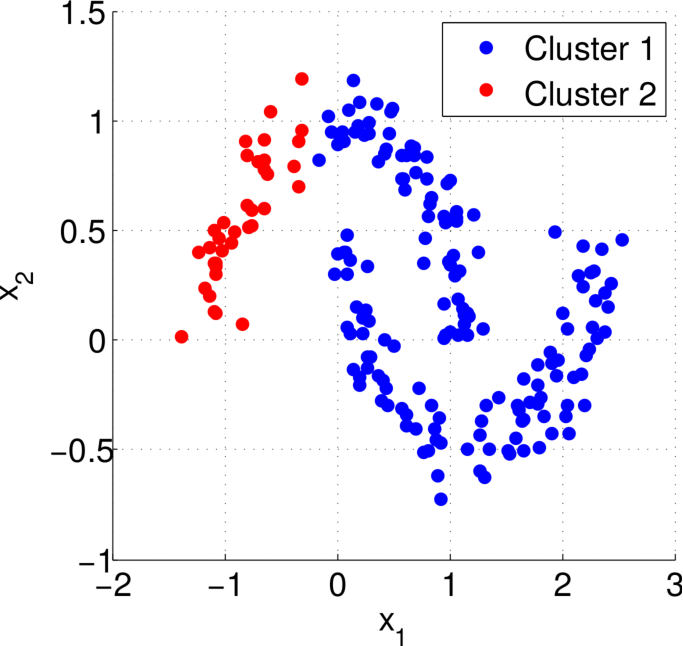
\includegraphics[width=5cm]{./figs/hw3_1_cluster_01.pdf}}
          \centerline{(c) Clustering.}\medskip
        \end{minipage}
        \caption{Clustering result for $\epsilon=0.1$.}
        \label{fig:hw3_1_01}
      \end{figure}
      
      \begin{figure}[htb]
        \centering
        \begin{minipage}[b]{0.32\columnwidth}
          \centering
          \centerline{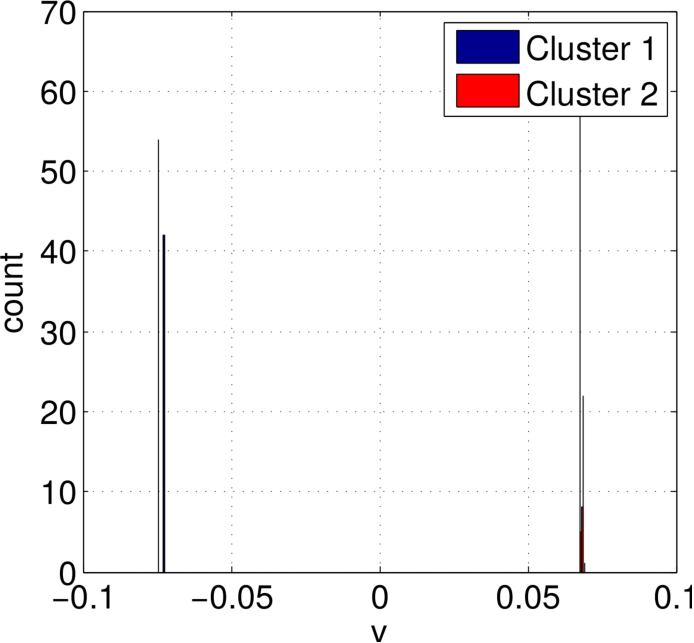
\includegraphics[width=5cm]{./figs/hw3_1_hist_001.pdf}}
          \centerline{(a) Histogram of $\mathbf{v}_2$.}\medskip
        \end{minipage}
        \hfill
        \begin{minipage}[b]{0.32\columnwidth}
          \centering
          \centerline{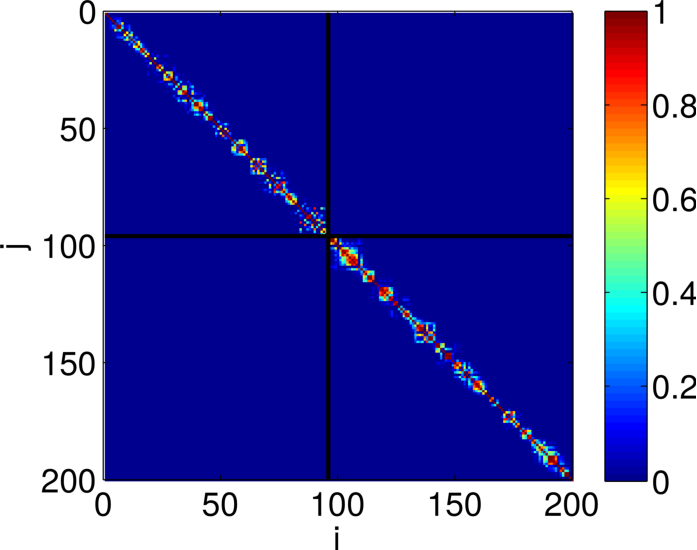
\includegraphics[width=6cm]{./figs/hw3_1_W_001.pdf}}
          \centerline{(b) $\mathbf{W}$ ordered and clustered.}\medskip
        \end{minipage}
        \hfill
        \begin{minipage}[b]{0.32\columnwidth}
          \centering
          \centerline{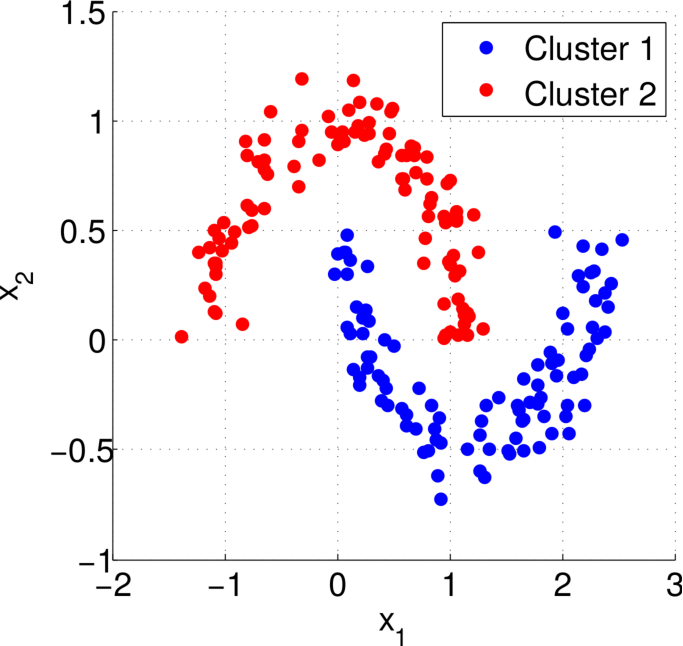
\includegraphics[width=5cm]{./figs/hw3_1_cluster_001.pdf}}
          \centerline{(c) Clustering.}\medskip
        \end{minipage}
        \caption{Clustering result for $\epsilon=0.01$.}
        \label{fig:hw3_1_001}
      \end{figure}

    }
    Source code:
\begin{lstlisting}[language=Matlab]
clear all;
close all;
clc;

load('crescents.mat');
[p, n] = size(x);
% figure;
% scatter(x(1,:), x(2, :))

epsilon = 0.01;
W = exp(-pdist2(x', x') .^ 2 / epsilon);

L = diag(sum(W)) - W;
[V, D] = eig(L);
v = real(V(:, 2));
idx = kmeans(v, 2);

figure;
scatter(x(1, idx == 1), x(2, idx == 1), [], 'MarkerEdgeColor', 'b', 'MarkerFaceColor', 'b'), hold on;
scatter(x(1, idx == 2), x(2, idx == 2), [], 'MarkerEdgeColor', 'r', 'MarkerFaceColor', 'r');
xlabel('x_1', 'fontsize', 16), ylabel('x_2', 'fontsize', 16);
legend('Cluster 1', 'Cluster 2')
set(gca, 'fontsize', 16);
grid on;

figure;
[n1,v1] = hist(v(idx == 1));
[n2,v2] = hist(v(idx == 2));
bar(v1, n1, 'hist')
hold on; 
h = bar(v2, n2, 'hist'); hold off
set(h,'facecolor','r');
legend('Cluster 1', 'Cluster 2');
xlabel('v', 'fontsize', 16), ylabel('count', 'fontsize', 16);
set(gca, 'fontsize', 16);
grid on;

[~, idx_sort] = sort(v);
figure;
imagesc(W(idx_sort, idx_sort)), hold on;
if idx(idx_sort(1)) == 1
    n_cluster1 = sum(idx == 1);
else
    n_cluster1 = sum(idx == 2);
end

plot(n_cluster1 * ones(1, n), 1 : n, 'k', 'linewidth', 2);
plot(1 : n, n_cluster1 * ones(1, n), 'k', 'linewidth', 2);
colorbar;
axis equal
set(gca, 'fontsize', 16);
xlim([0, 200]), ylim([0, 200]);
xlabel('i', 'fontsize', 16), ylabel('j', 'fontsize', 16);
\end{lstlisting}
  \end{homeworkProblem}
  %\clearpage
  
  %----------------------------------------------------------------------------------------
  % PROBLEM 2
  %----------------------------------------------------------------------------------------
  \begin{homeworkProblem}
    Download the dataset \texttt{genomedata.mat} from the Class website; it
    contains Single Nucleid Polymorphisms data from the Human Genome Diversity
    Project. The data consists of an array consisting of 5000 rows, each row has
    1043 different strings. The 5000 rows are Single Nucleid Polymorphisms, the
    columns correspond to 1043 different individuals. The entries are not
    numerical values (quite annoyingly), but contain the characters
    `AA', `CC', `GG', `TT', `AG', `AC', `TC', `TG', and (even more annoyingly)
    also `--', the latter represents missing measurements. Your goal is to
    cluster the data into a small set of clusters. After loading the file into
    Matlab, you need to convert the characters into numerical values. It is up
    to you which conversion you use (you can use the file \texttt{gen2vec.m} to
    do the actual conversion, once you have chosen a conversion rule).

    Since the data are high-dimensional you first need to reduce the dimension
    before clustering. You should attempt the dimension reduction via PCA as
    well as via diffusion maps. In both cases you need to decide how many
    dimensions you want to use. Also, in both cases you may want to use Matlab’s
    k-means function to do the actual clustering after dimension reduction.
    
    Note: Your results may differ from mine, because you will likely choose a
    different conversion rule. I did not get a meaningful clustering via PCA,
    but did achieve reasonable clustering via diffusion maps.
    \vspace{10pt}
      
    \problemAnswer{
      To cast the 9 possible character pairs into numerical values, we design
      the mapping on to the complex plane as shown in Fig.~\ref{fig:map}, which
      has the following desirable (heuristically) properties:
      \begin{itemize}
        \item The ``hybrid'' character pairs are close to their parental
        ``pure'' character pairs.
        \item The mappings are highly symmetric.
        \item '--' is not biased towards any non-empty character pair.
      \end{itemize}
      \begin{figure}[htb]
        \centering
        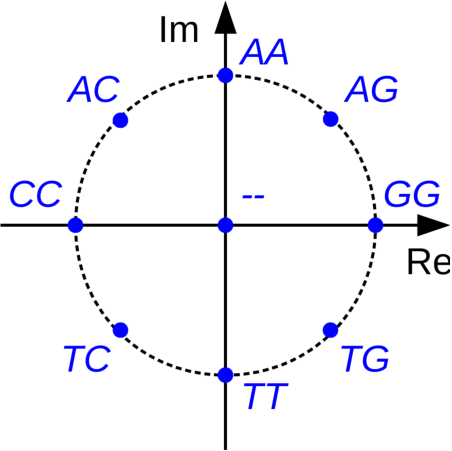
\includegraphics[width=0.2\columnwidth]{figs/map.pdf}
        \caption{Mapping the characters into numerical values (complex-valued).}
        \label{fig:map}
      \end{figure}
      
      To determine the number of clusters for k-means algorithm, the number of
      clusters $k$ is determined with Gap
      statistic~\cite{tibshirani2001estimating, hastie2005elements}, which
      selects $\hat{k}$ as the smallest $k$ producing a gap within one
      standard deviation of the gap at $k+1$.
      
      The dimension reduction and clustering results given by PCA are shown in
      Fig.~\ref{fig:hw3_2_pca}. As we can see, although the dimension of the
      data is high, there are only few large singular values (a). We select the
      first two principle components (complex-valued) and try to cluster them
      into 2 groups. The distributions of the real and imaginery parts for the 2
      clusters are shown in (c) which is not ideal. In (b) we can see that none
      of the $k\in[1, 10]$ satisfies the Gap statistic criterion,
      suggesting that PCA fails to provide a meaningful input to k-means.
      
      For diffusion maps we set the time scale $t=20$ and $\epsilon$ to be
      $1/10$ of the median of $\|\mathbf{x}_i - \mathbf{x}_j\|_2^2$. We reduce
      the dimension of the original data down to 3 so that a visualization is
      possible. As shown in Fig.~\ref{fig:hw3_2_dif}, based on the Gap
      statistic, the data should be clustered into 2 groups. And from the 3-D
      visualization and the scatter plot, the clustering is rather clear based
      solely on the first dimension.
      
      We also tried to cluster this data set with spectral clustering
      (unnormalized), which is closely related to diffusion maps. The results
      are shown in Fig.~\ref{fig:hw3_2_spec}. The Gap statistic suggest that
      $k=5$, though most data concentrates on two ``spikes'' as in the diffusion
      map approach.
      
      \begin{figure}[htb]
        \centering
        \begin{minipage}[b]{0.45\columnwidth}
          \centering
          \centerline{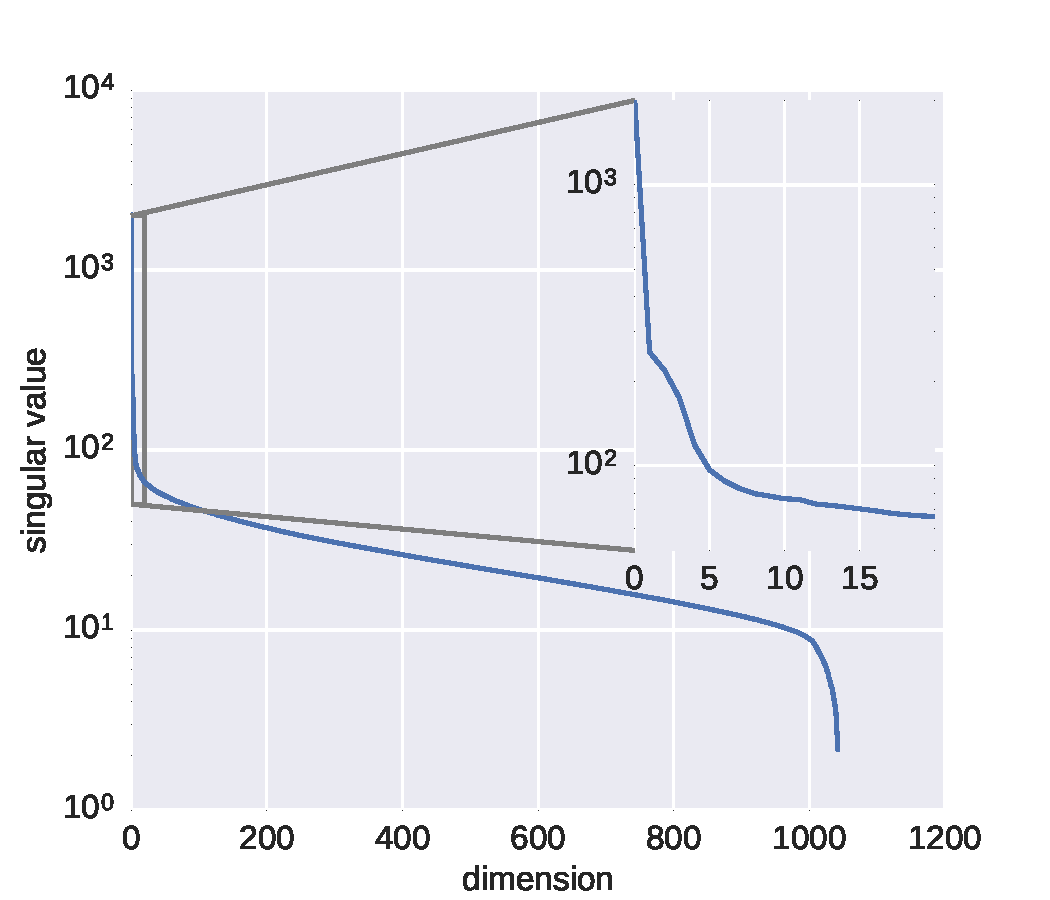
\includegraphics[width=8cm]{./figs/pca_singular.pdf}}
          \centerline{(a) Distribution of $\lambda$.}\medskip
        \end{minipage}
        \hfill
        \begin{minipage}[b]{0.45\columnwidth}
          \centering
          \centerline{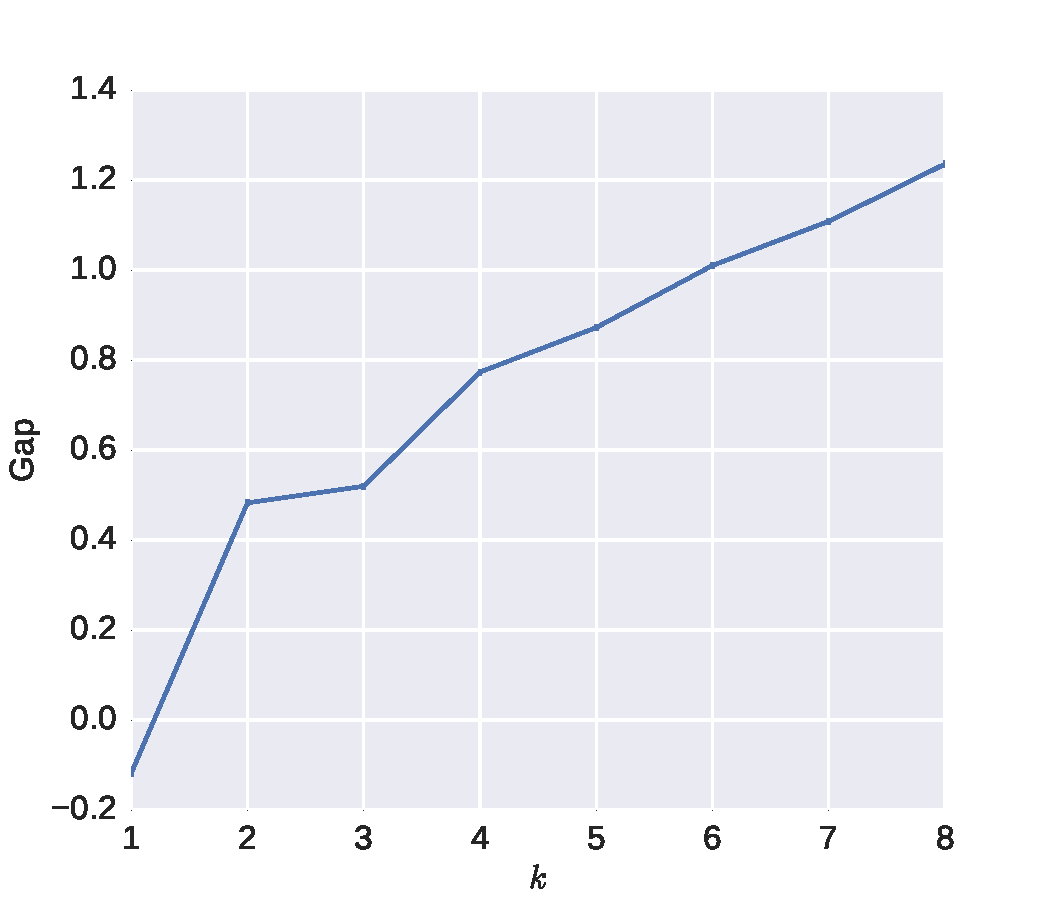
\includegraphics[width=8cm]{./figs/pca_gap.pdf}}
          \centerline{(b) Gap statistic.}\medskip
        \end{minipage}
        
        \centering
        \begin{minipage}[b]{0.7\columnwidth}
          \centering
          \centerline{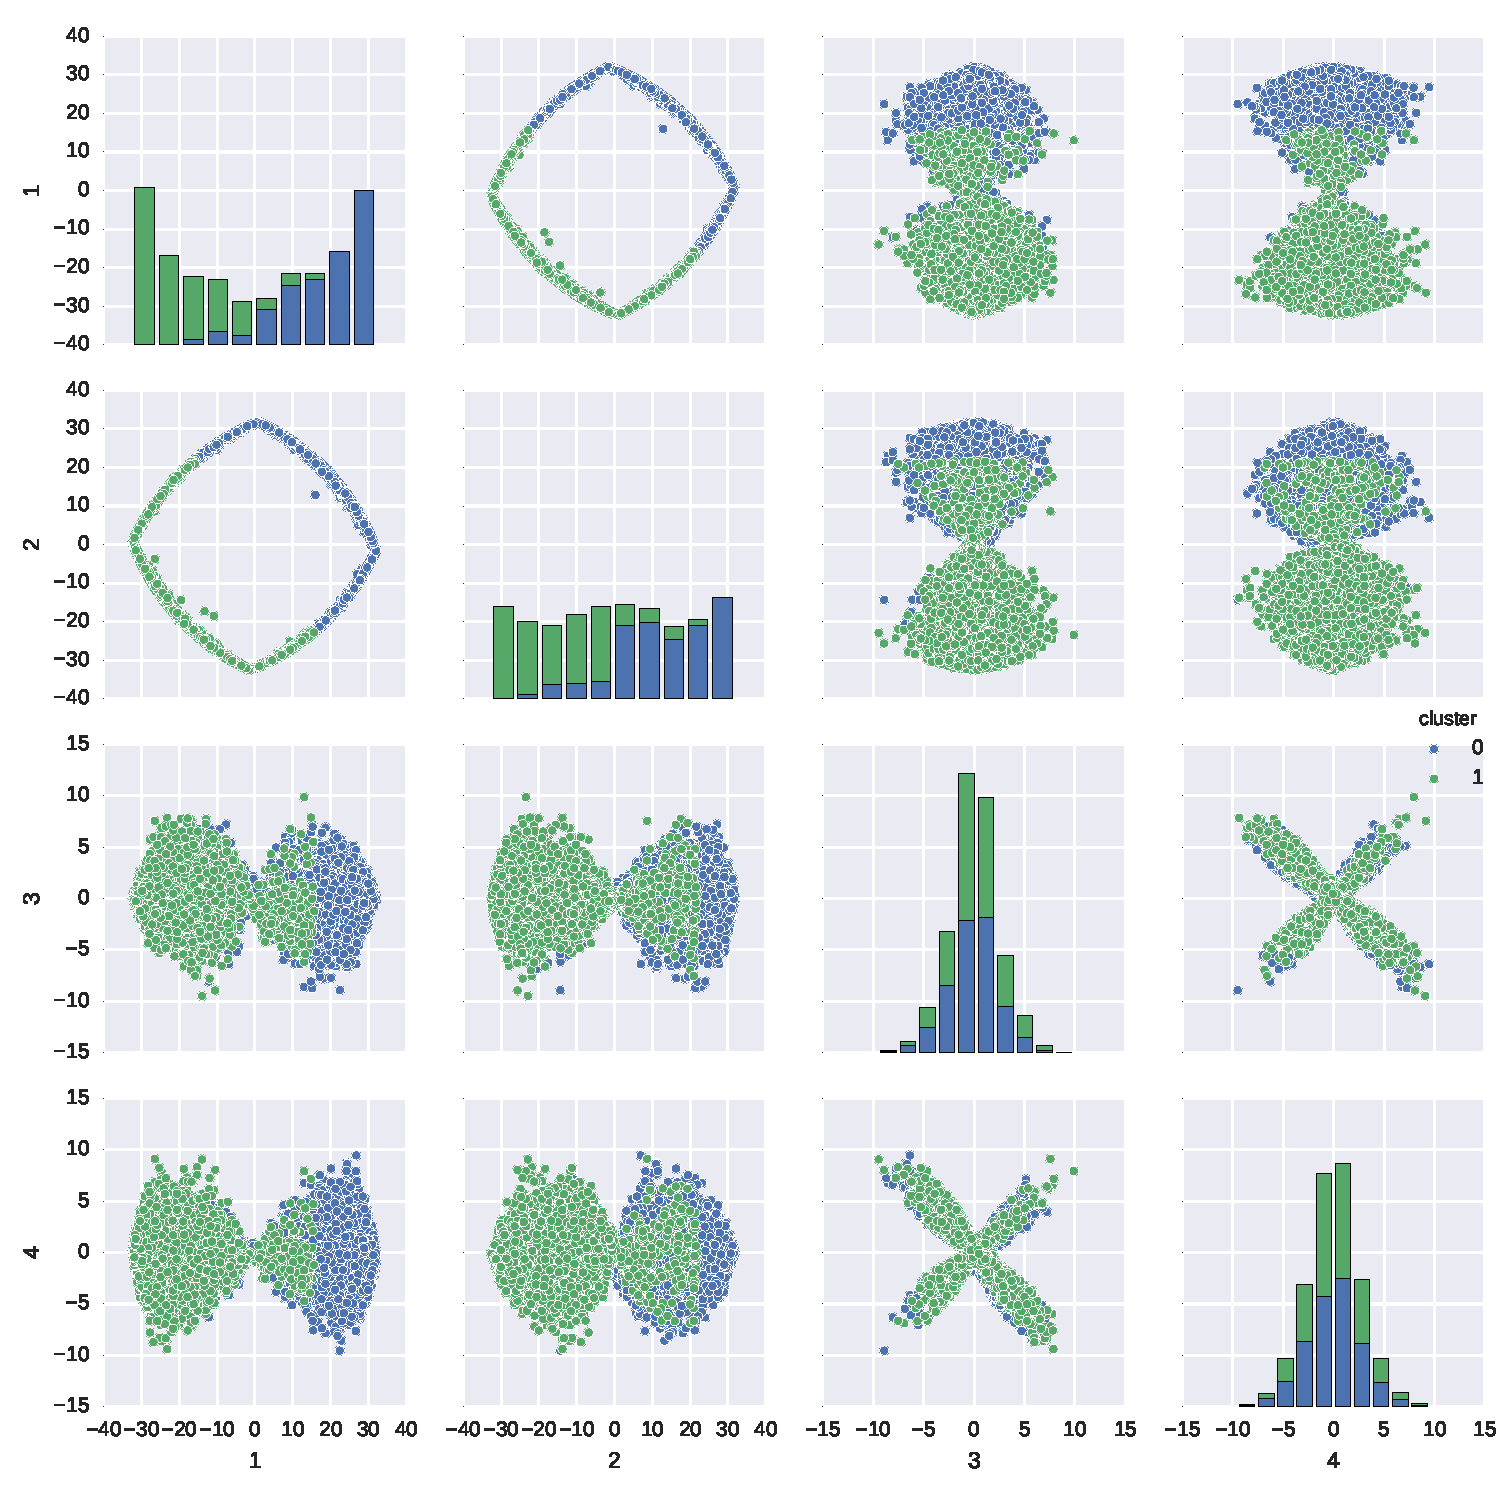
\includegraphics[width=10cm]{./figs/pca_scatter.pdf}}
          \centerline{(c) Scatter plot of the real and imaginery part
          of the first 2 principle components.}\medskip
        \end{minipage}
        \caption{Dimension reduction and clustering by PCA.}
        \label{fig:hw3_2_pca}
      \end{figure}
      
      \begin{figure}[htb]
        \centering
        \begin{minipage}[b]{0.45\columnwidth}
          \centering
          \centerline{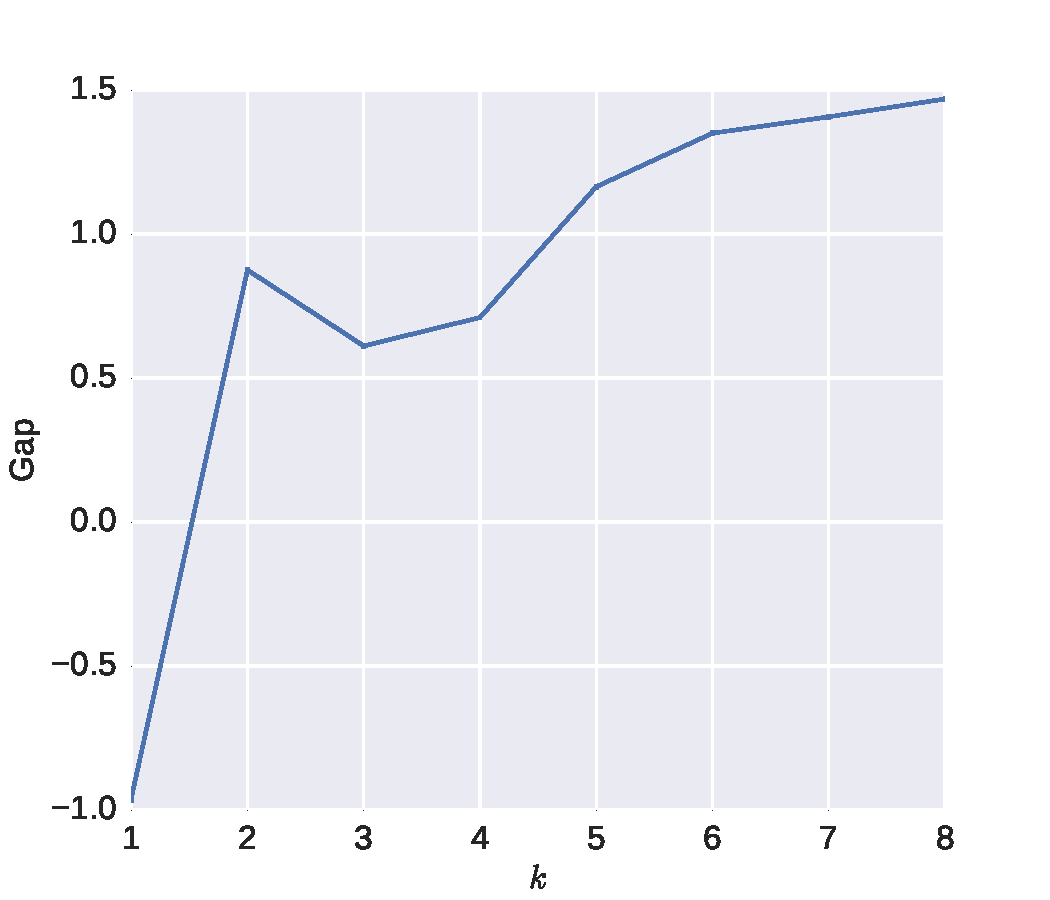
\includegraphics[width=8cm]{./figs/dif_gap.pdf}}
          \centerline{(a) Gap statistic.}\medskip
        \end{minipage}
        \hfill
        \begin{minipage}[b]{0.45\columnwidth}
          \centering
          \centerline{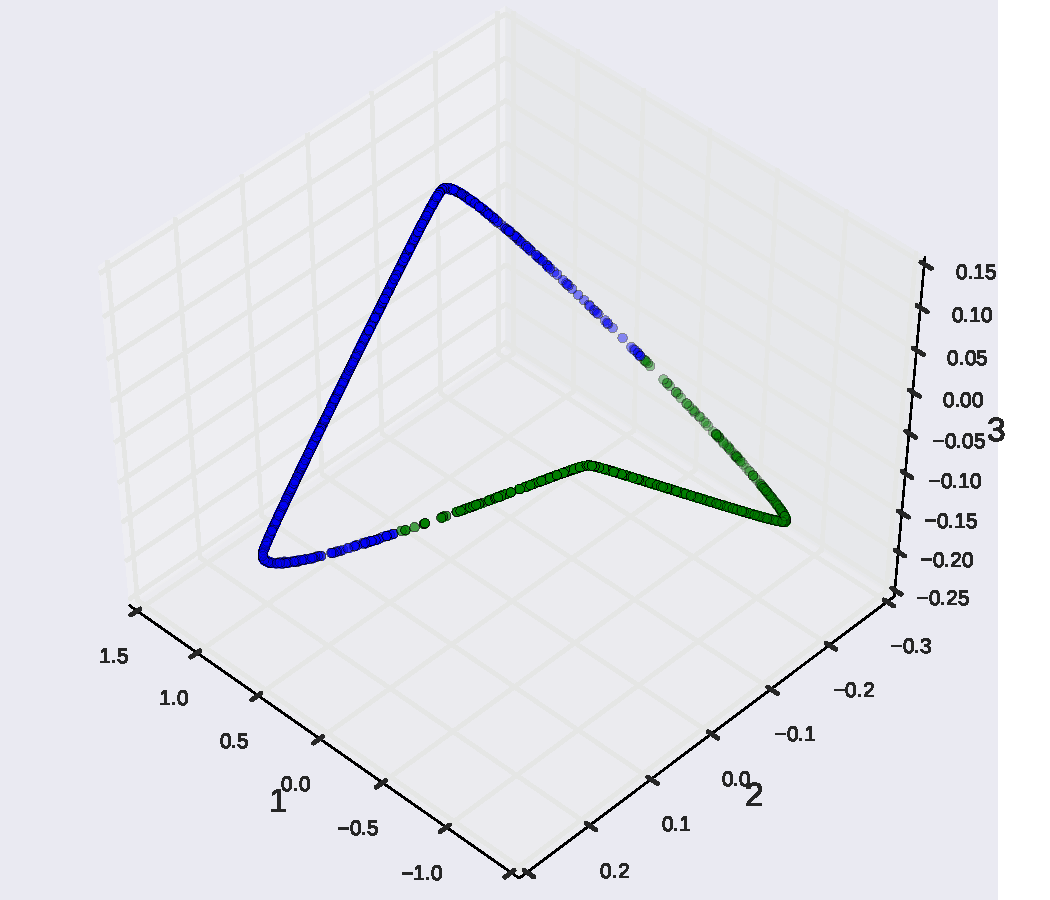
\includegraphics[width=7cm]{./figs/dif_3d.pdf}}
          \centerline{(b) 3-D visualization of the clustering.}\medskip
        \end{minipage}
        
        \centering
        \begin{minipage}[b]{0.7\columnwidth}
          \centering
          \centerline{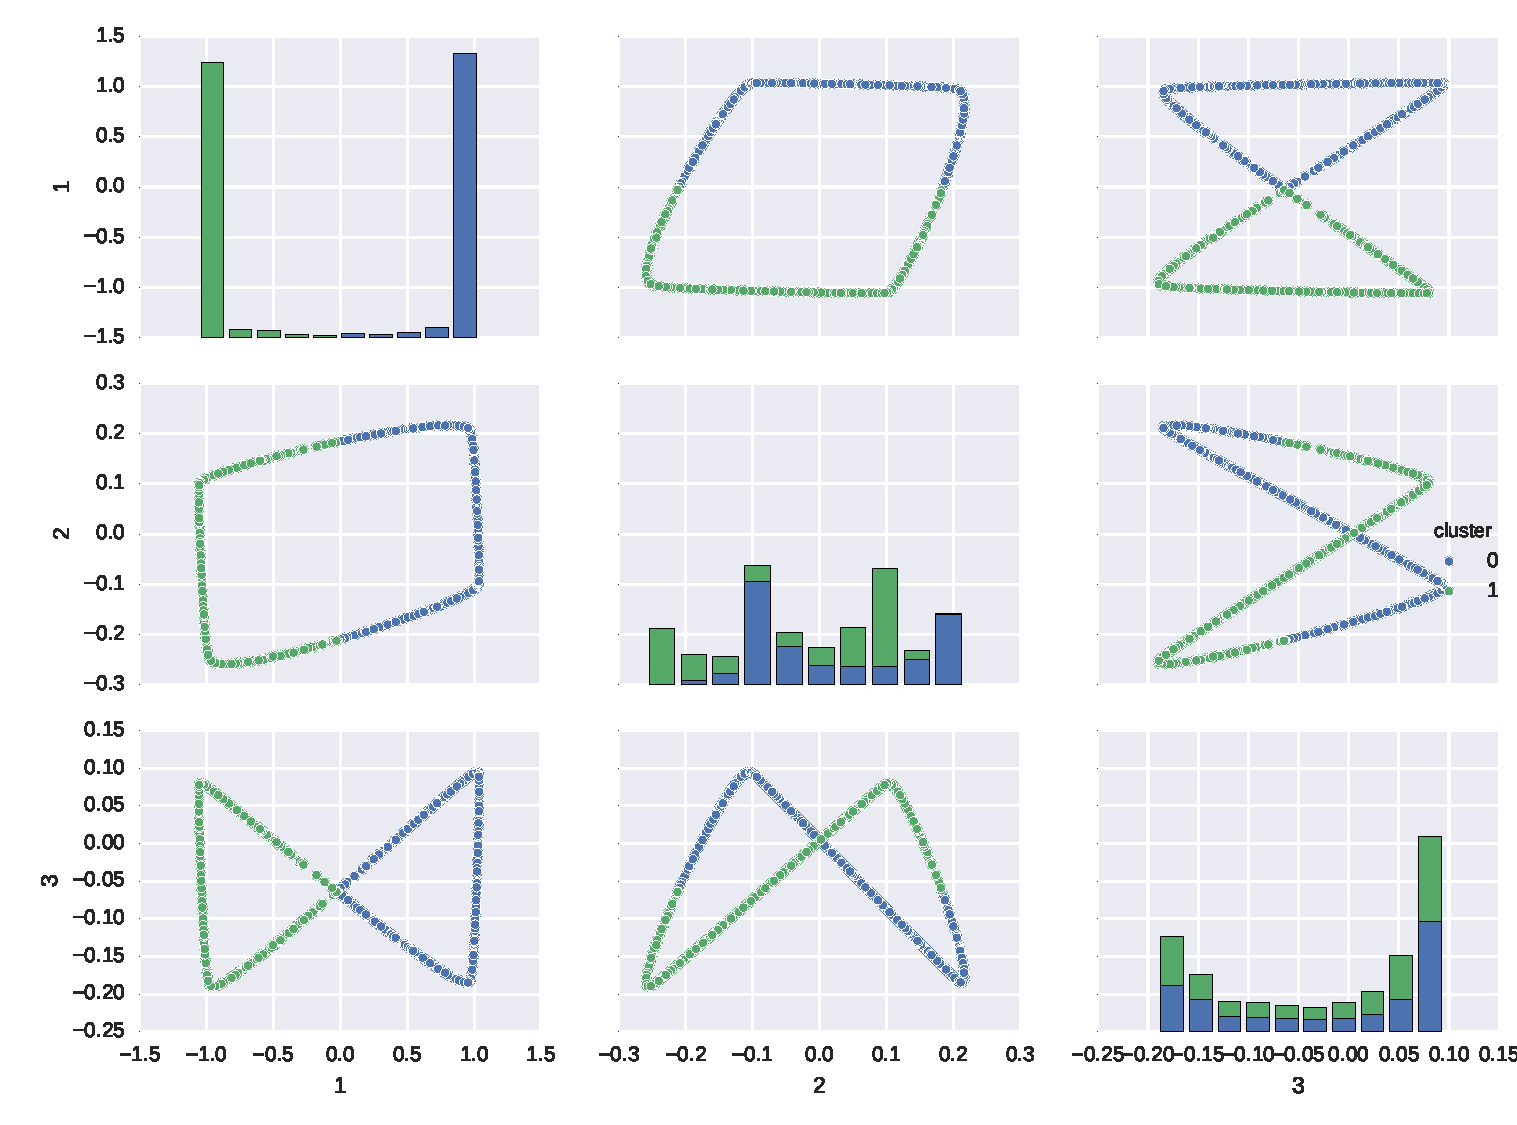
\includegraphics[width=10cm]{./figs/dif_scatter.pdf}}
          \centerline{(c) Scatter plot of the reduced dimension data.}\medskip
        \end{minipage}
        \caption{Dimension reduction and clustering by diffusion maps.}
        \label{fig:hw3_2_dif}
      \end{figure}
      
      \begin{figure}[htb]
        \centering
        \begin{minipage}[b]{0.45\columnwidth}
          \centering
          \centerline{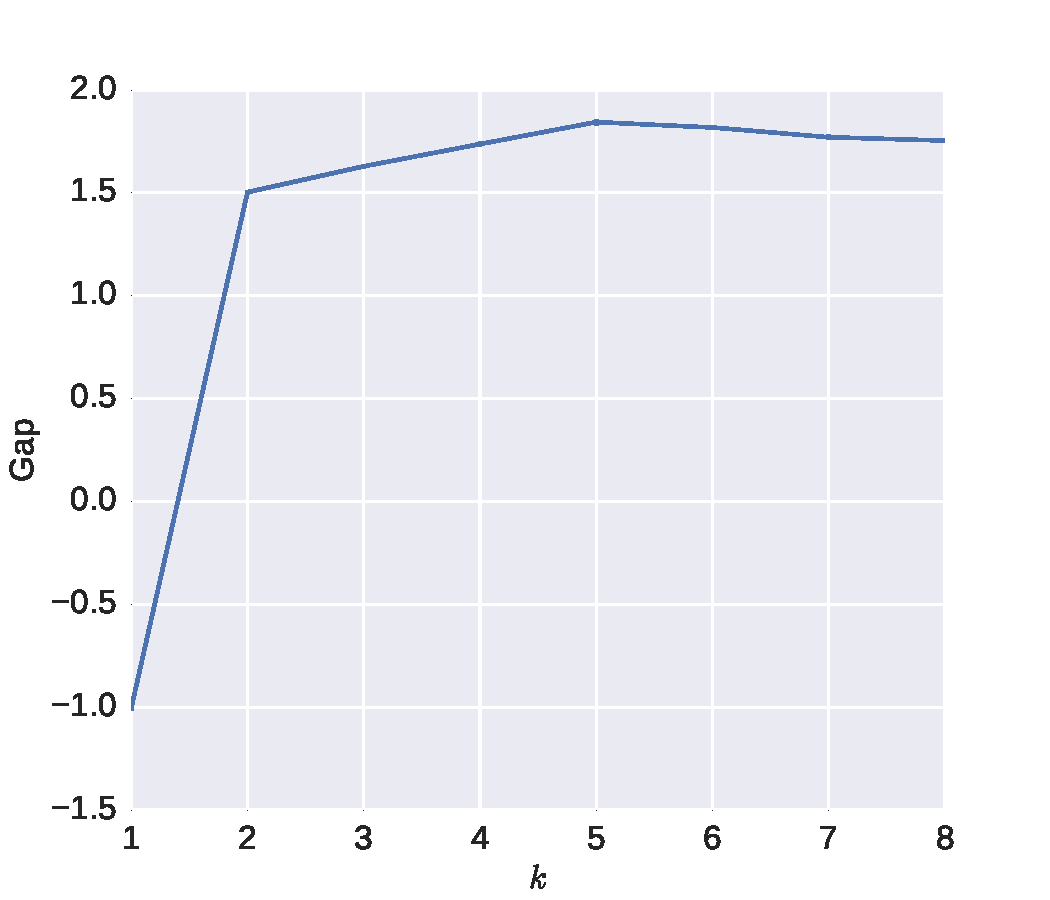
\includegraphics[width=8cm]{./figs/spec_gap.pdf}}
          \centerline{(a) Gap statistic.}\medskip
        \end{minipage}
        \hfill
        \begin{minipage}[b]{0.45\columnwidth}
          \centering
          \centerline{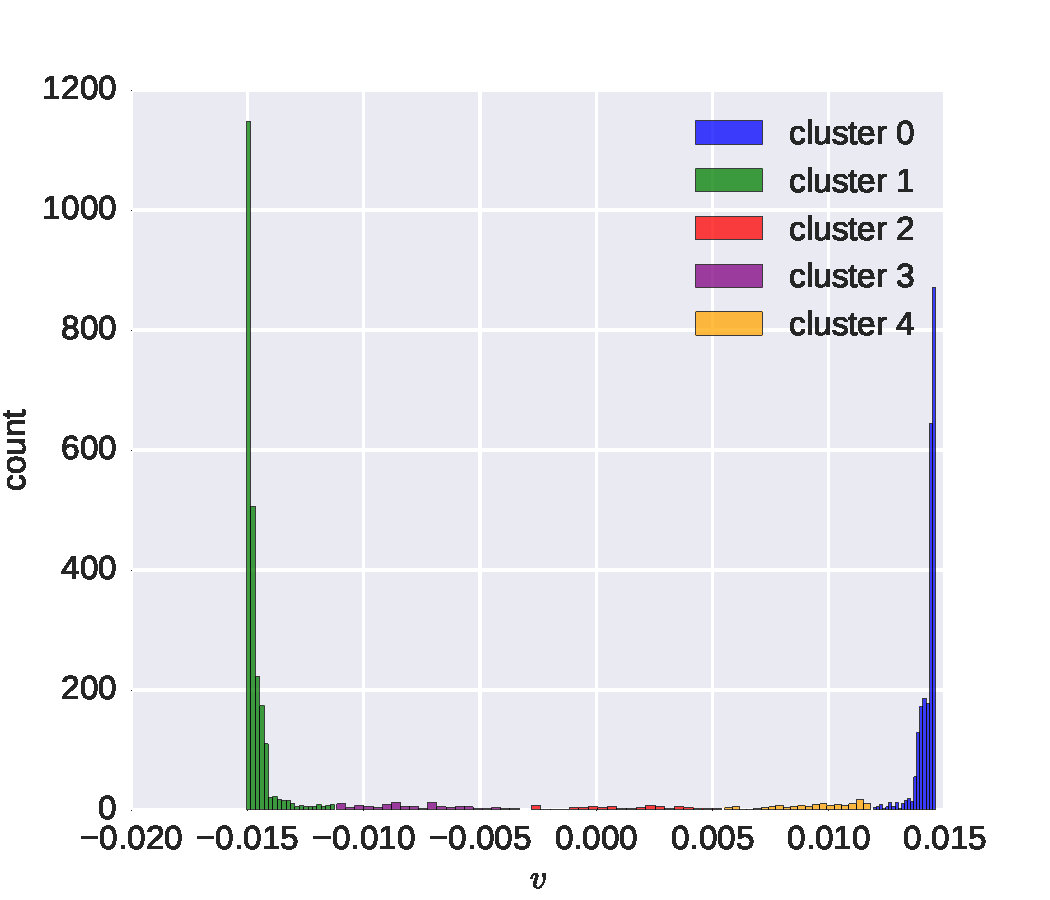
\includegraphics[width=8cm]{./figs/spec_hist.pdf}}
          \centerline{(b) Histogram of the second eigenvector of
          $\mathbf{L}$.}\medskip
        \end{minipage}
        \caption{Dimension reduction and clustering by spectral method.}
        \label{fig:hw3_2_spec}
      \end{figure}
    }
    Source code:
\begin{lstlisting}[language=Python]
import math
import cmath
import numpy as np
import pandas as pd
from numpy.linalg import svd
from numpy.random import uniform
from scipy import io
from scipy.linalg import eigh
from scipy.spatial.distance import pdist, squareform
from sklearn.cluster import KMeans

import matplotlib as mpl
import matplotlib.pyplot as plt
from mpl_toolkits.axes_grid1.inset_locator import inset_axes
from mpl_toolkits.axes_grid1.inset_locator import mark_inset
from mpl_toolkits.mplot3d import Axes3D
import seaborn as sns

%matplotlib qt
sns.set()
axis_font = {'size':'16'}
mpl.rcParams['xtick.labelsize'] = 16
mpl.rcParams['ytick.labelsize'] = 16

data = io.loadmat('genomedata.mat')
map_gen = {'AA': complex(0.0, 1.0),
           'CC': complex(-1.0, 0.0),
           'GG': complex(1.0, 0.0),
           'TT': complex(0.0, -1.0),
           'AG': complex(1.0 / math.sqrt(2), 1.0 / math.sqrt(2)),
           'AC': complex(-1.0 / math.sqrt(2), 1.0 / math.sqrt(2)),
           'TC': complex(-1.0 / math.sqrt(2), -1.0 / math.sqrt(2)),
           'TG': complex(1.0 / math.sqrt(2), -1.0 / math.sqrt(2)), 
           '--': complex(0.0, 0.0)}

X_raw = [[string.strip() for string in row[0][0].strip().split('\t')] for row in data['X']]
X = np.array([[map_gen[string] for string in row] for row in X_raw])
n, p = X.shape
X = X - np.mean(X, axis=0) * np.ones(p)

random_state = 8 # The random state used by the KMeans

# The function to evaluate the gap statistic for k-means with different number of clusters
def get_gapstat(X, k_range=np.arange(1, 9), n_sample=20, random_state=8):
    n, p = X.shape
    
    X_ref = np.empty((n, p, n_sample), dtype='float64')
    for col in range(p):
        X_ref[:, col, :] = uniform(low=X[:, col].min(), high=X[:, col].max(), size=(n, n_sample))
    
    gapstat = np.empty((n_sample, len(k_range)), dtype='float64')
    for i_k, k in enumerate(k_range):
        km = KMeans(n_clusters=k, random_state=random_state)
        
        # The inertia of the actual data
        km.fit(X)
        w = km.inertia_
        
        # The inertia of the reference data
        w_ref = np.empty(n_sample, dtype='float64')
        for i_sample in range(n_sample):
            km.fit(X_ref[:, :, i_sample])
            w_ref[i_sample] = km.inertia_
        
        gapstat[:, i_k] = np.log(w_ref) - np.log(w)
        
    return gapstat

k_range = np.arange(1, 9)
n_sample = 20

d_pca = 2 # For PCA we reduce the dimension of X down to 3
k_pca = 2 # The expected number of clusters for PCA

_, s_pca, V_pca = svd(X) # svd of X. Note that this is different from matlab in that X = U diag(s) V.
V_pca = np.conjugate(V_pca.T)

X_pca_complex = np.dot(X, V_pca[:, 0 : d_pca]) # Reduce the dimension of X by linear projection, a complex matrix

# Since KMeans does not seem to support complex value, expand the space to 2*d_pca dim
X_pca = np.empty((n, 2 * d_pca), dtype="float64") 
X_pca[:, 0::2] = X_pca_complex.real
X_pca[:, 1::2] = X_pca_complex.imag

label_pca = KMeans(n_clusters=2, random_state=random_state).fit_predict(X_pca)
gap_pca = get_gapstat(X_pca, k_range=k_range, n_sample=n_sample)

# Distribution of the sinular values
fig, ax = plt.subplots(figsize=(7, 6))
axins = inset_axes(ax, 2, 3, loc=1) # zoom-factor: 2.5, location: upper-left

ax.semilogy(np.arange(p), s_pca, linewidth=2)
ax.grid(True)
ax.set_xlabel('dimension', **axis_font)
ax.set_ylabel('singular value', **axis_font)

axins.semilogy(np.arange(p), s_pca, linewidth=2)
axins.grid(True)
x1, x2, y1, y2 = 0, 20, 50, 2000 # specify the limits
axins.set_xlim(x1, x2) # apply the x-limits
axins.set_ylim(y1, y2) # apply the y-limits
axins.set_xticks(np.arange(0, 20, 5))
mark_inset(ax, axins, loc1=2, loc2=3, fc="none", ec="0.5", lw=2)

fig.savefig('pca_singular.pdf', dpi=10)

# Scatterplot matrix
df_pca = pd.DataFrame({**{'cluster': label_pca}, **{col+1: X_pca[:, col] for col in range(2 * d_pca)}})
sns.pairplot(df_pca, hue='cluster', vars=np.arange(1, 1 + 2 * d_pca))
plt.savefig('pca_scatter.pdf', dpi=10)

# Gap statistics
fig, ax = plt.subplots(figsize=(7, 6))
ax.errorbar(k_range, np.mean(gap_pca, axis=0), yerr=np.sqrt(1+1/n_sample)*np.std(gap_pca, axis=0))
ax.grid(True)
ax.set_xlabel('$k$', **axis_font)
ax.set_ylabel('Gap', **axis_font)
fig.savefig('pca_gap.pdf', dpi=10)

d_dif = 3 # For PCA we reduce the dimension of X down to 3 for 3-D visualization
k_dif = 2 # The expected number of clusters for diffusion map
t_dif = 20 # The time scale for diffusion map
f = 10 # The factor used to set epsilon according to the median of the square pairwise Euclidean distance

distance = pdist(np.concatenate((X.real, X.imag), axis=1), 'euclidean');
epsilon = np.median(distance ** 2) / f;
W = np.exp(-squareform(distance) ** 2 / epsilon)
D_inv_sqrt = np.diag(1 / np.sqrt(np.sum(W, axis=1)))
MS = np.dot(np.dot(D_inv_sqrt, W), D_inv_sqrt) # The symmetric M matrix

l_dif, V_dif = eigh(MS, eigvals=(n-d_dif-1, n-2)) # Remember to ignore the largest eigen vector
l_dif, V_dif = l_dif[::-1], V_dif[:, ::-1] # The eigen value are now in descending order. 

X_dif = np.dot(np.dot(D_inv_sqrt, V_dif), np.diag(l_dif ** t_dif)) # The redued dimension map at time t

label_dif = KMeans(n_clusters=k_dif, random_state=random_state).fit_predict(X_dif)
gap_dif = get_gapstat(X_dif, k_range=k_range, n_sample=n_sample)

df_dif = pd.DataFrame({**{'cluster': label_dif}, **{col+1: 1000*X_dif[:, col] for col in range(d_dif)}})
plot_scatterplot = sns.pairplot(df_dif, hue='cluster', vars=np.arange(1, 1 + d_dif))
plt.savefig('dif_scatter.pdf', dpi=10)

fig = plt.figure(1, figsize=(7, 6))
plt.clf()
ax = Axes3D(fig, rect=[0, 0, .95, 1], elev=48, azim=134)
plt.cla()

y = np.choose(label_dif, ['b', 'g'])
ax.scatter(1000*X_dif[:, 0], 1000*X_dif[:, 1], 1000*X_dif[:, 2], c=y)
ax.set_xlabel('1', **axis_font)
ax.set_ylabel('2', **axis_font)
ax.set_zlabel('3', **axis_font)
fig.savefig('dif_3d.pdf', dpi=10)

# Gap statistics
fig, ax = plt.subplots(figsize=(7, 6))
ax.errorbar(k_range, np.mean(gap_dif, axis=0), yerr=np.sqrt(1+1/n_sample)*np.std(gap_dif, axis=0))
ax.grid(True)
ax.set_xlabel('$k$', **axis_font)
ax.set_ylabel('Gap', **axis_font)

fig.savefig('dif_gap.pdf', dpi=10)

k_spec = 5 # The expected number of clusters for spectral clustering

L = np.diag(sum(W)) - W
_, V_spec = eigh(L)
X_spec = V_spec[:, 1:2] # The reduced dimension data, simply the second smallest eigen vector of L
label_spec = KMeans(n_clusters=k_spec, random_state=random_state).fit_predict(X_spec)
gap_spec = get_gapstat(X_spec, k_range=k_range, n_sample=n_sample)

fig, ax = plt.subplots(figsize=(7, 6))

c = ['b', 'g', 'r', 'purple', 'orange']
for k in range(k_spec):
    ax.hist(X_spec[label_spec==k, 0], 20, facecolor=c[k], alpha=0.75, label='cluster {0}'.format(k))
ax.legend(loc=1, fontsize=16)
ax.set_xlabel('$v$', **axis_font)
ax.set_ylabel('count', **axis_font)
fig.savefig('spec_hist.pdf', dpi=10)

# Gap statistics
fig, ax = plt.subplots(figsize=(7, 6))
ax.errorbar(k_range, np.mean(gap_spec, axis=0), yerr=np.sqrt(1+1/n_sample) * np.std(gap_spec, axis=0))
ax.grid(True)
ax.set_xlabel('$k$', **axis_font)
ax.set_ylabel('Gap', **axis_font)
fig.savefig('spec_gap.pdf', dpi=10)
\end{lstlisting}    
  \end{homeworkProblem}
  
  %\newpage
  %\begin{appendices} 
  %\end{appendices}
  \bibliographystyle{unsrt}
  \bibliography{refs}
  
  %----------------------------------------------------------------------------------------

\end{document}